%%%%%%%%%%%%%%%%%%%%%%%%%%%%%%%%%%%%%%%%%%%%%%%%%%%%%%%%%%%%%%%%%%%%%%%%
%% Customizações do abnTeX2 (http://abnTeX2.googlecode.com)           %%
%% para a Universidade de Fortaleza						              %%
%%                                                                    %%
%% This work may be distributed and/or modified under the             %%
%% conditions of the LaTeX Project Public License, either version 1.3 %%
%% of this license or (at your option) any later version.             %%
%% The latest version of this license is in                           %%
%%   http://www.latex-project.org/lppl.txt                            %%
%% and version 1.3 or later is part of all distributions of LaTeX     %%
%% version 2005/12/01 or later.                                       %%
%%                                                                    %%
%% This work has the LPPL maintenance status `maintained'.            %%
%%                                                                    %%
%% The Current Maintainer of this work is Bruno Lopes                 %%
%%                                                                    %%
%% Project available on: https://github.com/bruno-unifor/unifortex2   %%
%%                                                                    %%
%% Further information about abnTeX2                                  %%
%% are available on http://abntex2.googlecode.com/                    %%
%%                                                                    %%
%%%%%%%%%%%%%%%%%%%%%%%%%%%%%%%%%%%%%%%%%%%%%%%%%%%%%%%%%%%%%%%%%%%%%%%%

%%%%%%%%%%%%%%%%%%%%%%%%%%%%%%%%%%%%%%%%%%%%%%%%%%%%%%%%%%%%%%%%%%%%%%%%
%% Customizações do abnTeX2 (http://abnTeX2.googlecode.com)           %%
%% para a Universidade de Fortaleza						              %%
%%                                                                    %%
%% This work may be distributed and/or modified under the             %%
%% conditions of the LaTeX Project Public License, either version 1.3 %%
%% of this license or (at your option) any later version.             %%
%% The latest version of this license is in                           %%
%%   http://www.latex-project.org/lppl.txt                            %%
%% and version 1.3 or later is part of all distributions of LaTeX     %%
%% version 2005/12/01 or later.                                       %%
%%                                                                    %%
%% This work has the LPPL maintenance status `maintained'.            %%
%%                                                                    %%
%% The Current Maintainer of this work is Bruno Lopes                 %%
%%                                                                    %%
%% Project available on: https://github.com/bruno-unifor/unifortex2   %%
%%                                                                    %%
%% Further information about abnTeX2                                  %%
%% are available on http://abntex2.googlecode.com/                    %%
%%                                                                    %%
%%%%%%%%%%%%%%%%%%%%%%%%%%%%%%%%%%%%%%%%%%%%%%%%%%%%%%%%%%%%%%%%%%%%%%%%

\documentclass[
    a4paper,          % Tamanho da folha A4
    12pt,             % Tamanho da fonte 12pt
    chapter=TITLE,    % Todos os capitulos devem ter caixa alta
    section=TITLE,    % Todas as secoes devem ter caixa alta
    oneside,          % Usada para impressao em apenas uma face do papel
    english,          % Hifenizacoes em ingles
    spanish,          % Hifenizacoes em espanhol
    brazil            % Ultimo idioma eh o idioma padrao do documento
]{abntex2}

% Importações de pacotes
\usepackage[brazil]{babel} 
\usepackage[utf8]{inputenc}                         % Acentuação direta
\usepackage[T1]{fontenc}                            % Codificação da fonte em 8 bits
\usepackage{graphicx}                               % Inserir figuras
\usepackage{amsfonts, amssymb, amsmath}             % Fonte e símbolos matemáticos
\usepackage{booktabs}                               % Comandos para tabelas
\usepackage{verbatim}                               % Texto é interpretado como escrito no documento
\usepackage{multirow, array}                        % Múltiplas linhas e colunas em tabelas
\usepackage{indentfirst}                            % Endenta o primeiro parágrafo de cada seção.
\usepackage{listings}                               % Utilizar codigo fonte no documento
\usepackage{xcolor}
\usepackage{microtype}                              % Para melhorias de justificação?
\usepackage[portuguese,ruled,lined]{algorithm2e}    % Escrever algoritmos
\usepackage{algorithmic}                            % Criar Algoritmos
%\usepackage{float}                                  % Utilizado para criação de floats
\usepackage{amsgen}
\usepackage{lipsum}                                 % Usar a simulação de texto Lorem Ipsum
%\usepackage{titlesec}                               % Permite alterar os títulos do documento
\usepackage{tocloft}                                % Permite alterar a formatação do Sumário
\usepackage{etoolbox}                               % Usado para alterar a fonte da Section no Sumário
\usepackage[nogroupskip,nonumberlist,acronym]{glossaries}                % Permite fazer o glossario
\usepackage{caption}                                % Altera o comportamento da tag caption
\usepackage[alf, abnt-emphasize=bf, bibjustif, recuo=0cm, abnt-etal-cite=3, abnt-etal-list=0,abnt-etal-text=it]{abntex2cite}  % Citações padrão ABNT
%\usepackage[bottom]{footmisc}                      % Mantém as notas de rodapé sempre na mesma posição
%\usepackage{times}                                 % Usa a fonte Times
\usepackage{mathptmx}                               % Usa a fonte Times New Roman
%\usepackage{lmodern}                               % Usa a fonte Latin Modern
%\usepackage{subfig}                                % Posicionamento de figuras
%\usepackage{scalefnt}                              % Permite redimensionar tamanho da fonte
%\usepackage{color, colortbl}                       % Comandos de cores
%\usepackage{lscape}                                % Permite páginas em modo "paisagem"
%\usepackage{ae, aecompl}                           % Fontes de alta qualidade
%\usepackage{picinpar}                              % Dispor imagens em parágrafos
%\usepackage{latexsym}                              % Símbolos matemáticos
%\usepackage{upgreek}                               % Fonte letras gregas
\usepackage{appendix}                               % Gerar o apendice no final do documento
\usepackage{paracol}                                % Criar paragrafos sem identacao
\usepackage{lib/unifortex2}		                    % Biblioteca com as normas da Unifor para trabalhos academicos
\usepackage{pdfpages}                               % Incluir pdf no documento
\usepackage{amsmath}                                % Usar equacoes matematicas

% Organiza e gera a lista de abreviaturas, simbolos e glossario
\makeglossaries

% Gera o Indice do documento
\makeindex


%%%%%%%%%%%%%%%%%%%%%%%%%%%%%%%%%%%%%%%%%%%%%%%%%%%%%
%%          Configuracoes do uniforTeX2            %%
%%%%%%%%%%%%%%%%%%%%%%%%%%%%%%%%%%%%%%%%%%%%%%%%%%%%%

% Opcoes disponiveis

%% Trabalho final de GRADUAÇÃO no qual a folha de aprovação será um arquivo PDF
%\trabalhoacademico{tccgraduacaoPDF}

%% Trabalho final de GRADUAÇÃO no qual a folha de aprovação será gerada pelo modelo UniforTEX
\trabalhoacademico{tccgraduacao}

%% Trabalho final de ESPECIALIZAÇÃO no qual a folha de aprovação será gerada pelo modelo UniforTEX
%\trabalhoacademico{tccespecializacao}

%% Trabalho final de MESTRADO no qual a folha de aprovação será gerada pelo modelo UniforTEX
%\trabalhoacademico{dissertacao}

%% Trabalho final de DOUTORADO no qual a folha de aprovação será gerada pelo modelo UniforTEX
%\trabalhoacademico{tese}

% Define se o trabalho eh uma qualificacao
% Coloque 'nao' para versao final do trabalho

%\ehqualificacao{nao}

% Remove as bordas vermelhas e verdes do PDF gerado
% Coloque 'sim' pare remover

\removerbordasdohyperlink{sim}

% Adiciona a cor Azul a todos os hyperlinks

\cordohyperlink{nao}

%%%%%%%%%%%%%%%%%%%%%%%%%%%%%%%%%%%%%%%%%%%%%%%%%%%%%
%%          Informação sobre a IES                 %%
%%%%%%%%%%%%%%%%%%%%%%%%%%%%%%%%%%%%%%%%%%%%%%%%%%%%%

\ies{Universidade de Fortaleza}
\iessigla{UNIFOR}
\centro{Centro de Ciências Tecnológicas}

%%%%%%%%%%%%%%%%%%%%%%%%%%%%%%%%%%%%%%%%%%%%%%%%%%%%%
%%        Informação para TCC de Graduacao         %%
%%%%%%%%%%%%%%%%%%%%%%%%%%%%%%%%%%%%%%%%%%%%%%%%%%%%%

\graduacaoem{Ciência da Computação}
\habilitacao{bacharel} % Pode colocar tambem 'licenciada'

%%%%%%%%%%%%%%%%%%%%%%%%%%%%%%%%%%%%%%%%%%%%%%%%%%%%%
%%     Informação para TCC de Especializacao       %%
%%%%%%%%%%%%%%%%%%%%%%%%%%%%%%%%%%%%%%%%%%%%%%%%%%%%%

\especializacaoem{}

%%%%%%%%%%%%%%%%%%%%%%%%%%%%%%%%%%%%%%%%%%%%%%%%%%%%%
%%         Informação para Dissertacao             %%
%%%%%%%%%%%%%%%%%%%%%%%%%%%%%%%%%%%%%%%%%%%%%%%%%%%%%

\programamestrado{Programa de Pós-Graduação em Informática Aplicada}
\nomedomestrado{Mestrado Acadêmico em Ciência da Computação}
\mestreem{Ciência da Computação}
\areadeconcentracaomestrado{Ciência da Computação}

%%%%%%%%%%%%%%%%%%%%%%%%%%%%%%%%%%%%%%%%%%%%%%%%%%%%%
%%               Informação para Tese              %%
%%%%%%%%%%%%%%%%%%%%%%%%%%%%%%%%%%%%%%%%%%%%%%%%%%%%%

\programadoutorado{Programa de Pós-Graduação em Informática Aplicada}
\nomedodoutorado{Doutorado em Saúde Coletiva}
\doutorem{Saúde Coletiva}
\areadeconcentracaodoutorado{Saúde Coletiva}

%%%%%%%%%%%%%%%%%%%%%%%%%%%%%%%%%%%%%%%%%%%%%%
%%  Informação relacionadas ao trabalho     %%
%%%%%%%%%%%%%%%%%%%%%%%%%%%%%%%%%%%%%%%%%%%%%%

\autor{João Paulo Cysne RUbio}
\titulo{A Contribuição dos Testes Automatizados para as Aplicações BPMS}
\data{2018}
\local{Fortaleza -- Ceará}

% Exemplo: \dataaprovacao{01 de Janeiro de 2017}
\dataaprovacao{01 de Janeiro de 2017}

%%%%%%%%%%%%%%%%%%%%%%%%%%%%%%%%%%%%%%%%%%%%%
%%     Informação sobre o Orientador       %%
%%%%%%%%%%%%%%%%%%%%%%%%%%%%%%%%%%%%%%%%%%%%%

\orientador{Pedro Porfirio Muniz Farias}
\orientadories{Universidade de Fortaleza - UNIFOR}
\orientadorcentro{Centro de Ciências Tecnológicas - CCT}
\orientadorfeminino{nao} % Coloque 'sim' se for do sexo feminino

%%%%%%%%%%%%%%%%%%%%%%%%%%%%%%%%%%%%%%%%%%%%%
%%      Informação sobre o Co-orientador   %%
%%%%%%%%%%%%%%%%%%%%%%%%%%%%%%%%%%%%%%%%%%%%%

% Deixe o nome do coorientador em branco para remover do documento

\coorientador{}
\coorientadories{Universidade Co-orientador - SIGLA}
\coorientadorcentro{Centro do Co-orientador - SIGLA}
\coorientadorfeminino{nao} % Coloque 'sim' se for do sexo feminino

%%%%%%%%%%%%%%%%%%%%%%%%%%%%%%%%%%%%%%%%%%%%%
%%      Informação sobre a banca           %%
%%%%%%%%%%%%%%%%%%%%%%%%%%%%%%%%%%%%%%%%%%%%%

% Atenção! Deixe o nome do membro da banca para remover da folha de aprovacao

% Exemplo de uso:
% \membrodabancadois{Prof. Dr. Fulano de Tal}
% \membrodabancadoisies{Universidade Estadual do Ceará - UECE}

\membrodabancadois{Membro da Banca Dois}
\membrodabancadoiscentro{Centro de Ciências e Tecnologia - CCT}
\membrodabancadoisies{Universidade do Membro da Banca Dois - SIGLA}

\membrodabancatres{Membro da Banca Três}
\membrodabancatrescentro{Centro de Ciências e Tecnologia - CCT}
\membrodabancatresies{Universidade do Membro da Banca Três - SIGLA}

\membrodabancaquatro{Membro da Banca Quatro}
\membrodabancaquatrocentro{Centro de Ciências e Tecnologia - CCT}
\membrodabancaquatroies{Universidade do Membro da Banca Quatro - SIGLA}

\membrodabancacinco{Membro da Banca Cinco}
\membrodabancacincocentro{Centro de Ciências e Tecnologia - CCT}
\membrodabancacincoies{Universidade do Membro da Banca Cinco - SIGLA}

\membrodabancaseis{Membro da Banca Seis}
\membrodabancaseiscentro{Centro de Ciências e Tecnologia - CCT}
\membrodabancaseisies{Universidade do Membro da Banca Seis - SIGLA}

\begin{document}

	% Elementos pré-textuais
	\imprimircapa
	\imprimirfolhaderosto{}
	%\imprimirfichacatalografica{elementos-pre-textuais/ficha-catalografica}
	%\imprimirerrata{elementos-pre-textuais/errata}

	%%%%%%%%%%%%%%%%%%%%%%%%%%%%%%%%%%%%%%%%%%%%%%%%%%%%%%%%%%%%%%%%%%%%%%%%%%%%%%%%%%%%%%%%%%%%%%%%%%
	%%																                               	%%
	%%		Após a defesa do TCC, a banca examinadora irá preencher a folha de aprovação,			%%
	%%		que deverá ser assinada por todos os membros da banca avaliadora e, posteriormente,		%%
	%%		deverá ser anexada na versão final do TCC pelo ALUNO.									%%
	%%																								%%
	%%		Quando tiver em mãos a folha de aprovação:												%%
	%%			1 - Escanei-a e gere um arquivo PDF													%%
	%%			2 - Renomeie o arquivo PDF para "folha-aprovacao.pdf"								%%
	%%			3 - Mova o arquivo para o diretório "elementos-pre-textuais" do modelo				%%
	%%			5 - Descomente a linha 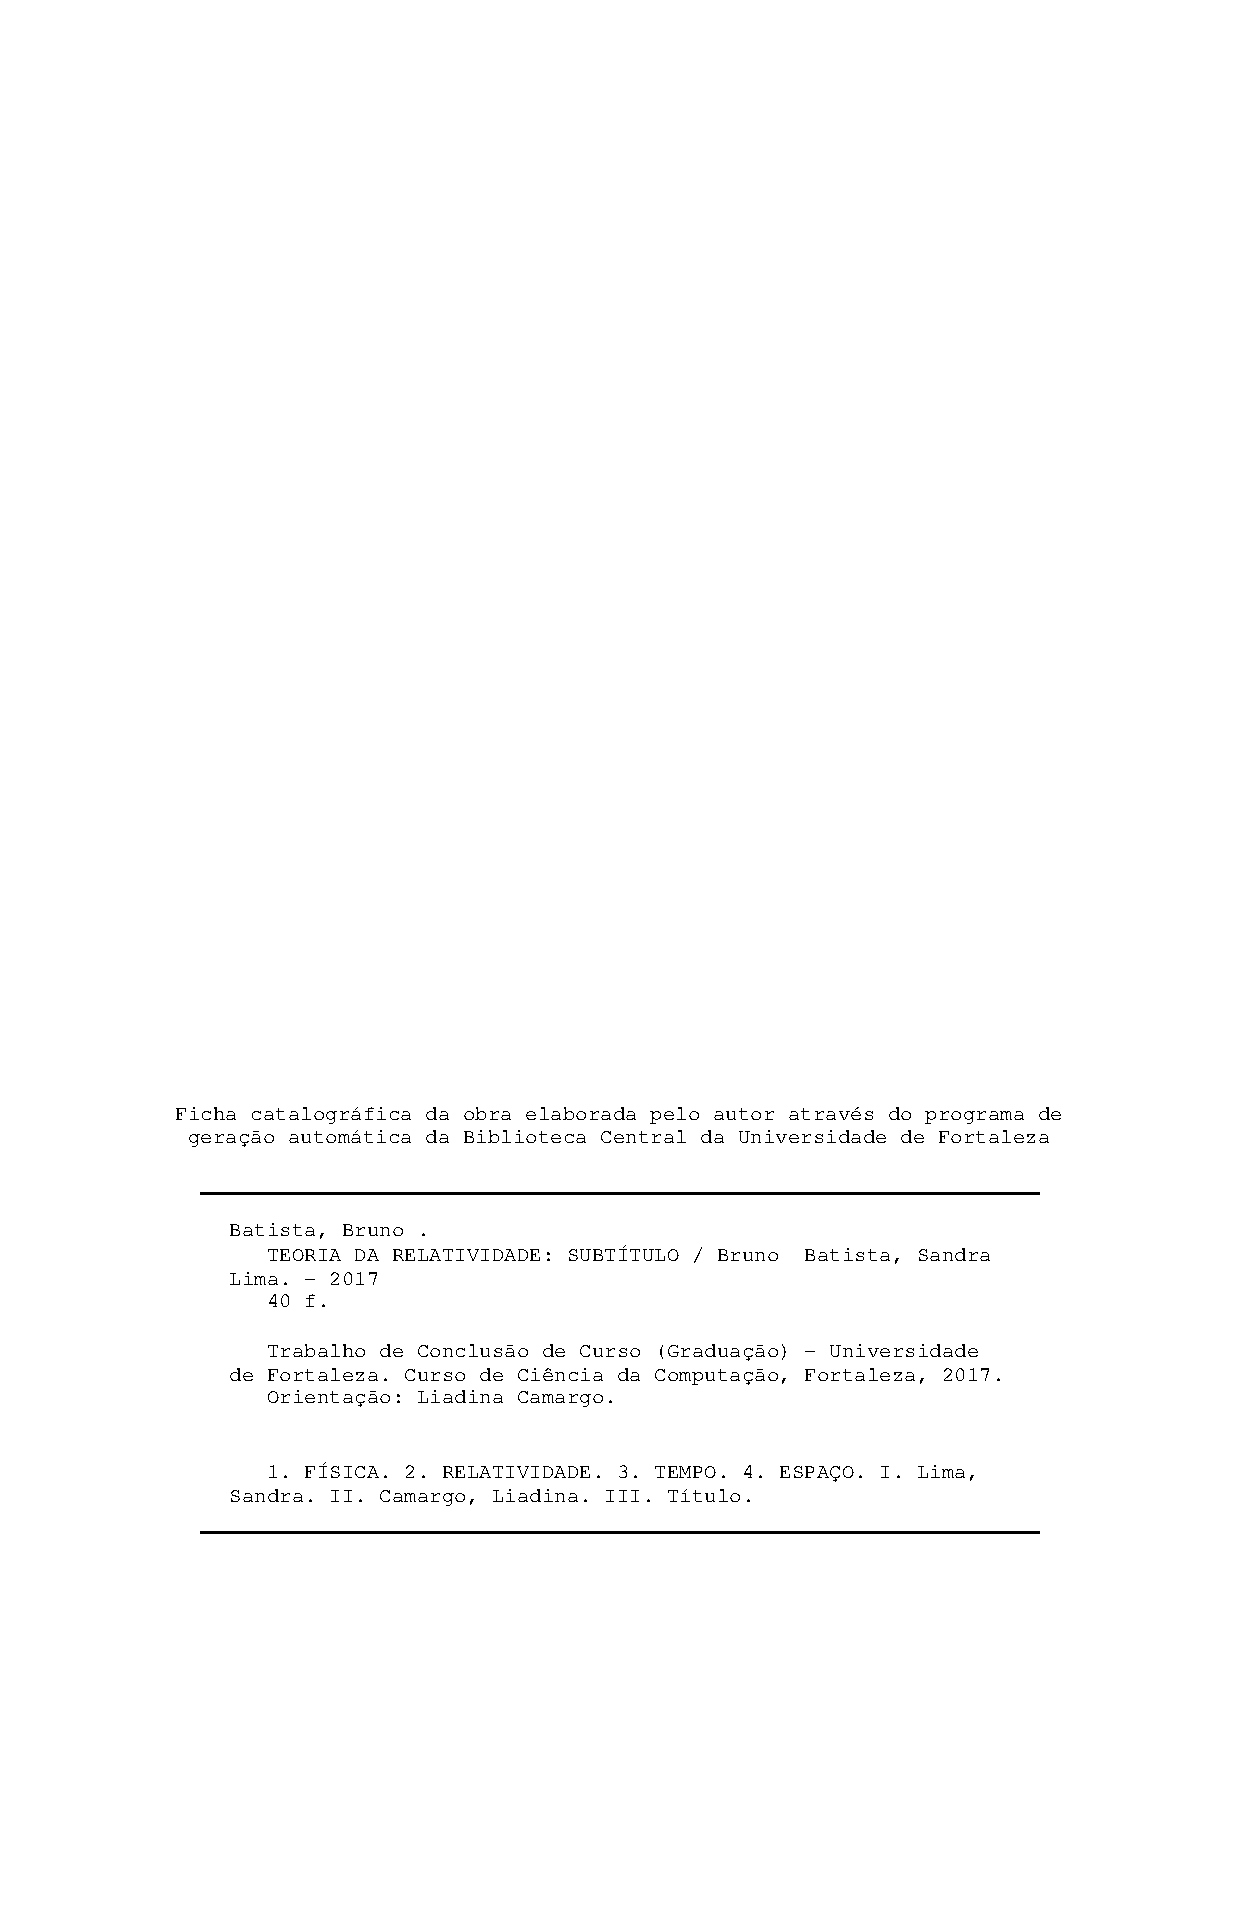
\includepdf{elementos-pre-textuais/folha-aprovacao.pdf} 		%%
	%%					removendo o simbolo de %													%%
	%%			6 - Adicione o simbolo % na linha 	\imprimirfolhadeaprovacao						%%
	%%			7 - Recompile o projeto																%%
	%%																								%%	%%%%%%%%%%%%%%%%%%%%%%%%%%%%%%%%%%%%%%%%%%%%%%%%%%%%%%%%%%%%%%%%%%%%%%%%%%%%%%%%%%%%%%%%%%%%%%%%%%
	
	%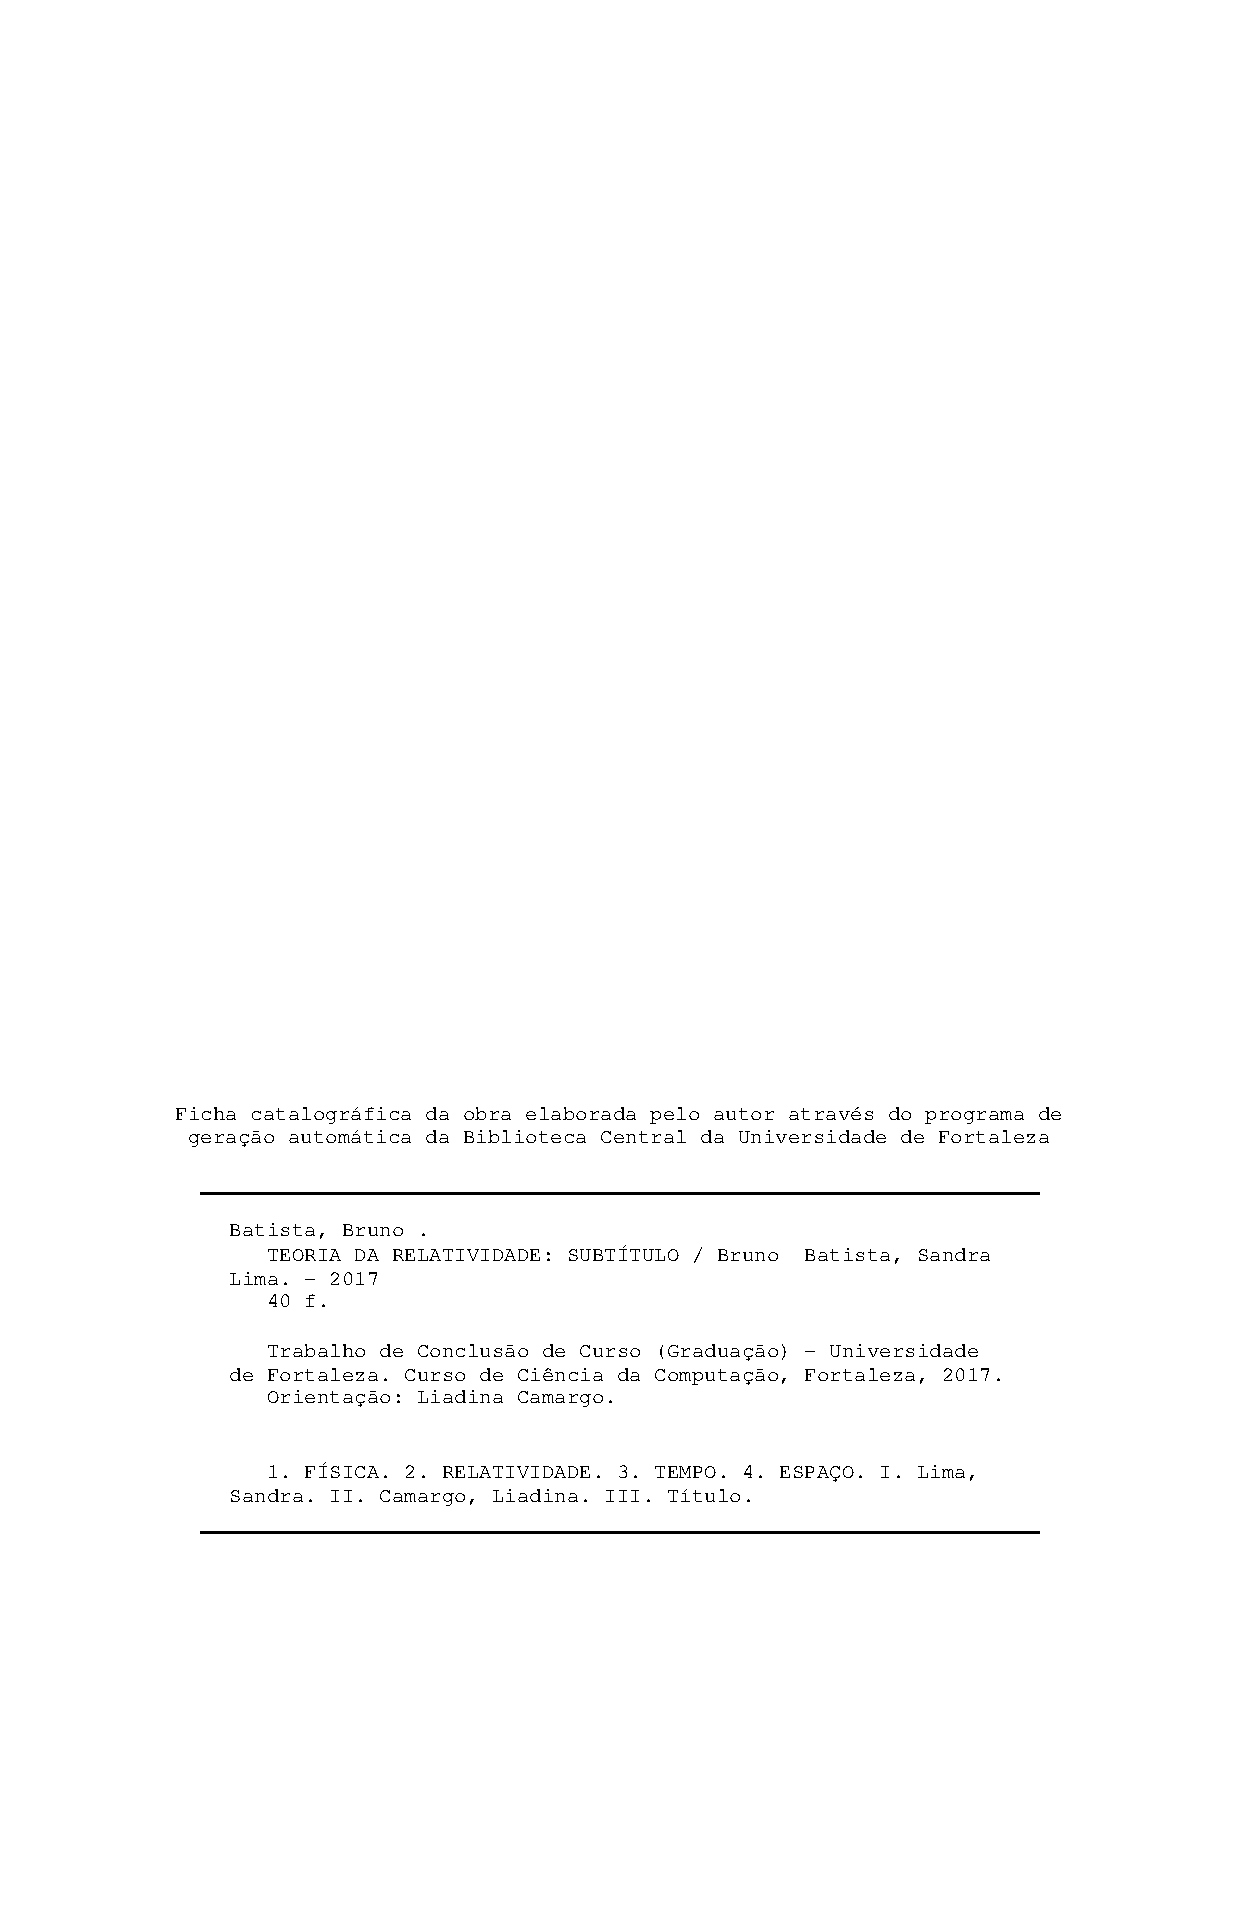
\includepdf{elementos-pre-textuais/folha-aprovacao.pdf}
	%\imprimirfolhadeaprovacao
	
	%\imprimirdedicatoria{elementos-pre-textuais/dedicatoria}
	\imprimiragradecimentos{elementos-pre-textuais/agradecimentos}
	%\imprimirepigrafe{elementos-pre-textuais/epigrafe}
	\imprimirresumo{elementos-pre-textuais/resumo}
	\imprimirabstract{elementos-pre-textuais/abstract}
	\imprimirlistadeilustracoes
	%\imprimirlistadetabelas
	%\imprimirlistadequadros
	%\imprimirlistadealgoritmos
	%\imprimirlistadecodigosfonte
	\imprimirlistadeabreviaturasesiglas
	%\imprimirlistadesimbolos{elementos-pre-textuais/lista-de-simbolos}
	\imprimirsumario

	%Elementos textuais
	\textual
	\chapter{Introdução}
\label{cap:introducao}

\lipsum[5]
\lipsum[6]
\lipsum[7]

\section{Motivação}
\label{sec:motivacao}

\lipsum[3]
\lipsum[4]

\section{Objetivos}
\label{sec:objetivos}

Interdum et malesuada fames ac ante ipsum primis in faucibus. Lorem ipsum dolor sit amet, consectetur adipiscing elit. Ut ex tellus, sodales in euismod at, ultricies quis leo.

\subsection{Objetivo Geral}
\label{sec:objetivo-geral}

Integer imperdiet ac magna eu pulvinar. Aliquam erat volutpat. Etiam molestie, nulla a egestas aliquet, velit augue congue metus, et ultricies metus massa vel nibh. Vivamus viverra commodo finibus. Nam elementum convallis accumsan. Quisque tincidunt purus nisl, tincidunt ultricies odio ultrices eu.

\subsection{Objetivos Específicos}
\label{sec:objetivos-especificos}

Lorem ipsum dolor sit amet, consectetur adipiscing elit. Duis scelerisque, velit at facilisis hendrerit, dui eros lacinia metus, non maximus mi tortor ut lectus. Donec hendrerit leo ut consectetur tincidunt. 

	\begin{alineas}
		\item Lorem ipsum dolor sit amet, consectetur adipiscing elit. Nunc dictum sed tortor nec viverra.
		\item Praesent vitae nulla varius, pulvinar quam at, dapibus nisi. Aenean in commodo tellus. Mauris molestie est sed justo malesuada, quis feugiat tellus venenatis.
		\item Praesent quis erat eleifend, lacinia turpis in, tristique tellus. Nunc dictum sed tortor nec viverra.
		\item Mauris facilisis odio eu ornare tempor. Nunc dictum sed tortor nec viverra.
		\item Curabitur convallis odio at eros consequat pretium.
	\end{alineas}
	\chapter{Introdução ao teste automatizado com ênfase nos tipos de testes}
\label{cap:Introdução ao teste automatizado com ênfase nos tipos de testes}

\section{Conceito sobre Testes Automatizados}
\label{sec:Conceito sobre Testes Automatizados}
	
	A área de teste de software tem crescido bastante nos últimos anos pelo fato de ter um aumento nas pesquisas e profissionais da área de teste de software. Esse aumento tem a ver com o crescimento rápido dos software e a exigência da entrega de software com menos problemas e mais qualidade \cite{LivroAutomatizacao}.
    
    O teste de software tem como proposta mostrar que o software desenvolvido faz oque foi prometido fazer e serve também para encontrar problemas antes do software ser utilizado pelo usuário final\cite{EngSofSommerville}. Alem disso, os testes feitos em um software não implica que o mesmo se encontra livre de problemas ou o software vai agir de acordo com as especificações feitas em qualquer momento \cite{EngSofSommerville}.
    
    Os testes automatizados são testes que são executado por uma ferramenta que contém vários item de teste. Onde esses testes são executados por meio do controladores de testes, que é um modulo de software que invoca um módulo sob teste. Além do mais, fica promovendo entradas de testes, monitorando a execução do teste ,controlando o mesmo e por fim, relata os resultados \cite{EngdeSoftwareFMP}.
    
    As vantagens de se usar os testes automatizado, são a economia do tempo que teria caso o teste fosse feito de forma manual e  diminui os problemas que são encontrado durante o desenvolvimento do sistema \cite{LivroAutomatizacao}. Por causa desse motivo, o teste automatizado é considerado indispensável nos dias de hoje para o desenvolvimento, pois só ele executam vários teste com grande volume de forma confiável para assim poder agilizar essa atividade \cite{EngdeSoftwareFMP}.  
    
    O código de teste que é criado para fazer os testes automatizado é semelhante ao codigo de uma aplicação, sendo algumas vezes superior. Além do mais esse codigo de teste tem que ser confiável, pelo motivo que vai ser utilizado para fazer os testes \cite{EngdeSoftwareFMP}. 
    
    A automatização dos testes não são totalmente automatizado uma vez que só testa aquilo que foi planejado. Por outro lado, oque os testes automatizados não fazem é testar como as coisas estão ,exemplo seria a interface do sistema \cite{EngSofSommerville}.
    
    
    
    
	Na Figura 1 encontram-se os tipos de testes usados quando se quer implementar um teste automatizado no seu software.  
    \begin{figure}[h!]
	\centering
		\Caption{\label{fig:Sequencia_de_Testes} Testes }	
		\UNIFORfig{}{
			\fbox{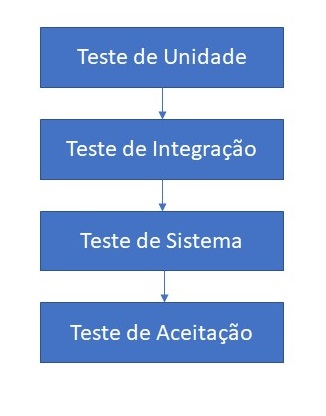
\includegraphics[width=8cm]{figuras/Sequencia_de_Testes.jpg}}
		}
       	{
			\Fonte{Elaborado pelo autor}
		}	
	\end{figure}
    
\subsection{Teste de unidade}
\label{sec:Teste de unidade}
	O teste de unidade é executado em todo o ciclo de vida do desenvolvimento do software, onde é testados as menores unidades componentes do sistema que são considerados: as classes, as funções e objetos do sistema. Onde se considera a performance do sistema e a lógica do usada no sistema. Nesse testes se usasse de parâmetros diferentes de entrada, para mostrar a existência do erro em cada componentes do sistema testado. Além disso, o teste de unidade pode ser usado como técnica para teste de caixa preta e caixa branca. No qual o teste de caixa preta pode ser aplicado na fase de desenvolvimento, mas o teste de caixa branca é o teste mais frequente a ser utilizado. \cite{ReginaldoRe} 
    
    Quando é executado o teste de unidade nas classes de objetos, os testes devem ser projetados para garantir a abrangência de todas as características do objeto \cite{EngSofSommerville}. Segundo o \cite{EngSofSommerville} deve-se "Testar todas as operações associadas ao objeto; Definir e verificar o valor de todos os atributos associados ao objeto; Colocar o objeto em todos os estados possíveis, oque significa simular todos os eventos que causam mudanças de estado;".
    
    %A herança, nas classes de objetos, é considerada complexa quando submetido a um teste de unidade. Pelo motivo de que, quando é testado uma operação na classe principal não se pode assumir que essa operação vai funcionar correto nas subclasses que herdaram essa operação. Por causa disso, é indispensável testar as operações nas subclasses que herdaram essa operação para todos os testes dessa operação\cite{EngSofSommerville}.
    
    %O testes de unidade automatizados são executado com o uso de \textit{framework} para testes(como JUnit, Selenion...), onde se desenvolve scripts que tem classes de testes genéricas ou pode ter classes de testes especificas, que quando executadas os testes criados nos scripts é informado por uma interfase gráfica se os testes deram certo ou deram errado. Com um conjunto de scripts de teste sendo executado em um \textit{framework}, o tempo para executar os testes pode ser em pouco segundo.\cite{EngSofSommerville}
    
    %Com o uso de ferramentas como JUnit, o desenvolvimento das classes de teste fica mais simples de implementar e executar os testes que foram pedidos. Contudo, existe um grande desafio em implementar as classes de testes, pelo fato de exigir um conhecimento de programação e de testes. \cite{UsingRulestoSupportSoftwareTesting}  
    
    


\subsection{Teste de integração}
\label{sec:Teste de integração}
	O teste de integração tem como definição um teste que verifica os componentes do sistema e testa cada um dos componentes. \cite{EngdeSoftwareFMP}. Onde verifica problemas envolvendo a construção do software. Consequentemente é uma técnica sistemática para a construção da arquitetura do software, onde simultaneamente realia os testes para encontrar problemas relacionados as interfaces do sistema \cite{pressman}.
    
    
    Dentro do teste de integração existem duas estrategias que são "bottom-up" e "top-down". Onde o "bottom-up" baseia-se em testar os módulos de baixo nível até chegar nos módulos de alto nível e o "top-down" é o inverso do "bottom-up" \cite{CidinhaCostaGouveia}.
	
    A estratégia top-down aborda a construção da arquitetura do software de forma incremental, onde os módulos são integrados e move-se para baixo por meio de uma hierarquia de controle que é iniciado com o módulo de controle principal. Os módulos subordinados ao módulo de controle principal são agregados de duas possíveis  formas na estrutura de hierarquia de controle: depth-first(primeiro-em-profundidade), onde faz a integração em todos os componentes criando um caminho de controle principal na estrutura do programa e breadth-first(primeiro-em-largura), onde junta todos os componentes subordinados a cada nível e move esses componentes através da estrutura horizontalmente. \cite{pressman}.
    
    Já a estratégia bottom-up aborda o inicio da construção e o teste com os módulos atômicos( nível mais baixo da estrutura do sistema). Onde os componentes são constituídos de baixo para cima, com isso proporciona o componentes subordinados a certos niveis estarem sempre disponíveis e a exigência de pseudocontroladores não vai existir \cite{pressman}.
   
    Quando o teste de integração é realizado, existe a possibilidade de que o mesmo afete o teste de unidade e o  também afete o custo dos testes. Por causa dos erros encontrados durante o teste de integração, pode provocar correções nas unidades testadas no teste de unidade. Onde vai implicar na correção da unidade e em um novo uso dos teste de unidade e de integração. Portando o teste de integração deve ser usado no começo do desenvolvimento junto com o teste de unidade. Se usando disso, ajuda a conter os custo de manutenção nas fases finais do desenvolvimento e contribui para o melhoramento da qualidade dos testes de unidade. \cite{MARLLOSPAIVAPRADO} 
    
    
    
    
\subsection{Teste de sistema}
\label{sec:Teste de sistema}
	O teste de sistema tem como foco verificar todo o sistema, para confirmar se todos os requisitos do software foi feito de forma correta. Onde nesse teste, é considerado todos as funcionalidades que são importante para o funcionamento do sistema, como : segurança, performance e robustez\cite{LivroAutomatizacao}.
    Acrescentando-se que, esse teste precisa aprovar os requisitos funcionas do software e  também precisa validar os requisitos não funcionais que foram estabelecidos \cite{ReginaldoRe}. Ademais esse teste aprova o sistema quando ele é integrado a um sistema maior \cite{pressman}.
    

    

    
    
    
    
    
\subsection{Teste de aceitação}
\label{sec:Teste de aceitação}
	O teste de aceitação é executado junto com o cliente com ou não supervisão dos desenvolvedores. Alem disso nesse teste, todo o sistema é testado pelo cliente para verificar a existência de erros. Após o teste, o cliente relata aos desenvolvedores os error que foram tidos no teste\cite{LivroAutomatizacao}. 
    Além do mais, esse teste é para garantir que o software cumpra todos os requistos funcionais, comportamentais e de desempenho estalecidos \cite{pressman}.
    
    Acrescentando-se que esse teste pode ser feito em um períodos longos (semanas ou meses), para assim descobrir erros cumulativos, que podem prejudicam o sistema \cite{pressman}. 
    
    
    
    


\chapter{Introdução a ferramenta BPMS com ênfase em sua arquitetura}
\label{cap:Introdução a ferramenta BPMS com ênfase em sua arquitetura}
Como mencionado antes uma ferramenta BPMS suporta as notações do BPMN e tem as disciplinas gerenciais do BPM dentro da ferramenta. A ferramenta BPMS tem origem em ferramentas de workflow que foram evoluindo ao longo do tempo, onde houve a junção de motores de regras de negocio e geração de aplicação na ferramenta de workflow. Assim as aplicações criadas dentro do BPMS são geradas e acessas por dentro do BPMS\cite{CBOK}.

O BPMS criou um nível de automação que possibilitou a junção dos modelos de negócios com regras e as informações que tem nas atividades do processo. Além disso,a ferramenta possou capacidade de gerir e criar aplicações somente como os modelos junto com as suas regras. Assim oferecendo um gerenciamento do fluxo do trabalho\cite{CBOK}.

As ferramentas BPMS dificilmente são parecidas, já que elas envolve diferentes etapas do ciclo de vida do BPM: onde os sistemas mais simples só envolver a parte de design dos processos e a automação do mesmo, já os sistemas mais complexo tem oque o sistema simples tem e contem o SOA, integrações com sistema de terceiros, Processamento de Eventos (CEP) e por fim, inteligencia do processo \cite{ProcessAwareBPM}.

Com o uso do SOA(Service-oriented architecture) ajudou os BPMS a fazerem integrações com os sistemas legados, onde o SOA é uma adaptador junto com web services para se comunicar com sistemas legados. Os BPMS utilizam-se dessa arquitetura para se comunicar com os outros sistemas das organizações e assim tirando proveito dessa camada nos processos criados \cite{CBOK}.

Devido a competição entre fornecedores, ocorre uma evolução dos BPMS e consequentemente, uma corrida para fornecer o melhor ambiente para a operação, conduzindo assim uma rápida expansão de sua capacidade e melhoria geral de sua qualidade e estabilidade, essa evolução direciona-se em duas categorias. As ferramentas autônomas, que por seu custo mais baixo, facilita às organizações, a capacidade de análise e definição de seus processos e fluxos de trabalho, assim como análise de regras de negócio, e muitas vezes, a descoberta de inconsistências e conflitos. Outra categoria consiste nos grupos integrados de ferramentas, que evoluíram para a geração de aplicações capazes de prover suporte à lógica complexa e transações em alto volume \cite{CBOK}.


\section{Arquitetura do BPMS}
\label{sec:Arquitetura do BPMS}
	Na Figura a baixo podemos ver como é divido a Arquitetura de uma ferramenta BPMS
    
\begin{figure}[h!]
	\centering
		\Caption{\label{fig:SOA} Arquitetura do BPMS }	
		\UNIFORfig{}{
			\fbox{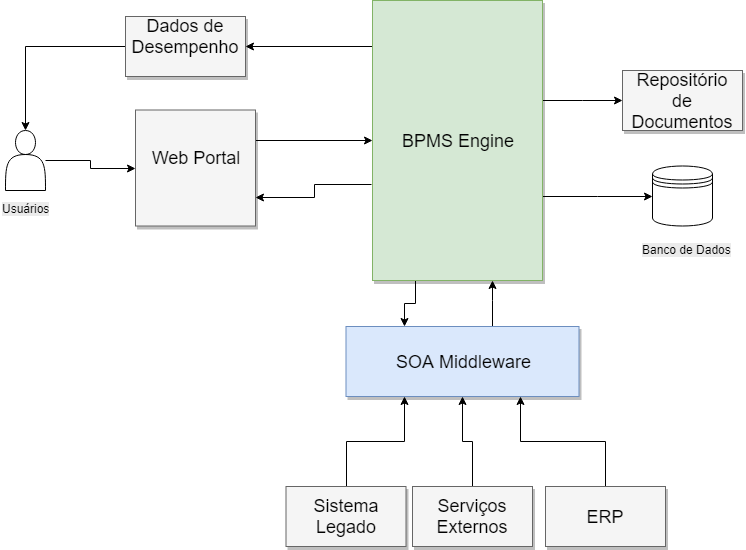
\includegraphics[width=15cm]{figuras/BPMS__Arquitetura.png}}
		}
       	{
			\Fonte{Elaborado pelo autor}
		}	
	\end{figure}
    
    \textbf{BPMS Engine }: considerado o coração do BPMS, é a parte do BPMS que tem diferentes funcionalidades que podem ser a seguintes: criação de processos executáveis (Cases), distribuição das atividades para os participantes do processo, capacidade de recuperar e guardar os dados necessários para executar o processo, executar atividades automatizadas para diferente tipos de software, criação e modificação de modelos de processos, criação do modelo de dados usado nos processos, capacidade de criar formulários e mantém o controle das atividades que estão perto de terminar o tempo.   \cite{ProcessAwareBPM}.
    
    \textbf{SOA Middleware}: é uma middleware que é usado no desenvolvimento de aplicações e integrações com diferentes tipos de sistemas \cite{CBOK}. O SOA se conecta com diferentes serviços para obter dados requerido pelo processo na aplicação BPMS.
    
    \textbf{Web Portal}: Portal que mostra ao usuário quando o mesmo entra na aplicação. Nesse portal o usuário poderá: criar cases(instância de um processo), fazer buscas e administrar os processo.  
    
    %é um conjunto flexível de princípios de desenho de infraestrutura usados no desenvolvimento de aplicações e integração de sistemas.
    



%	\begin{figure}[h!]
%		\centering		\Caption{\label{fig:}  }	
%		\UNIFORfig{}{
%			\fbox{\includegraphics[width=8cm]{figuras/}}
%		}{
%			\Fonte{}			
%		}	
%	\end{figure}
















	%\chapter{Trabalhos Relacionados}
\label{cap:trabalhos-relacionados}



\section{Trabalho Relacionado A}
\label{sec:trabalho-relacionado-a}



	


\section{Trabalho Relacionado B}
\label{sec:trabalho-relacionado-b}


	\chapter{Metodologia}
\label{chap:metodologia}

\lipsum[2]
\lipsum[12]

O autor \cite{lamport1986latex} e \cite{Maia2011} \lipsum[2] 

\begin{table}[h!]
	\Caption{\label{tabela-ibge} Um Exemplo de tabela alinhada que pode ser longa ou curta, conforme padrão IBGE}%
	\IBGEtab{}{%
		\begin{tabular}{ccc}
			\toprule
			Nome & Nascimento & Documento \\
			\midrule \midrule
			Maria da Silva & 11/11/1111 & 111.111.111-11 \\
			Maria da Silva & 11/11/1111 & 111.111.111-11 \\
			Maria da Silva & 11/11/1111 & 111.111.111-11 \\
			\bottomrule
		\end{tabular}%
	}{%
	\Fonte{Produzido pelos autores}%
	\Nota{Esta é uma nota, que diz que os dados são baseados na
		regressão linear.}%
	\Nota[Anotações]{Uma anotação adicional, seguida de várias outras.}%
}
\end{table}

\cite{Huetal2000} \lipsum[2] 

\section{Exemplo de Algoritmos e Figuras}
\label{sec:exemplo-de-algoritmos-e-figuras}

\lipsum[2]

\begin{algorithm}[h!]
	\SetSpacedAlgorithm
	\caption{\label{exemplo-de-algoritmo}Como escrever algoritmos no \LaTeX2e}
	\Entrada{o proprio texto}
	\Saida{como escrever algoritmos com \LaTeX2e }
	\Inicio{
		inicializa\c{c}\~ao\;
		\Repita{fim do texto}{
			leia o atual\;
			\Se{entendeu}{
				vá para o próximo\;
				próximo se torna o atual\;}
			\Senao{volte ao início da seção\;}
		}
	}	
\end{algorithm}

\lipsum[2]
%\begin{algorithm}[H]
%	\Entrada{o proprio texto}
%	\Saida{como escrever algoritmos com \LaTeX2e }
%	\Inicio{
%		inicializa\c{c}\~ao\;
%		\Repita{fim do texto}{
%			leia o atual\;
%			\Se{entendeu}{
%				vá para o próximo\;
%				próximo se torna o atual\;}
%			\Senao{volte ao início da seção\;}
%		}
%	}
%	\caption{Exemplo de Algoritmo Versao 02}
%\end{algorithm}

%\begin{algorithm}
%	\begin{algorithmic}
%	\Entrada{o proprio texto}
%	\Saida{como escrever algoritmos com \LaTeX2e }	
%	\end{algorithmic}
%\end{algorithm}

Exemplo de alíneas com números:

\begin{alineascomnumero}
	\item Lorem ipsum dolor sit amet, consectetur adipiscing elit. Nunc dictum sed tortor nec viverra.
	\item Praesent vitae nulla varius, pulvinar quam at, dapibus nisi. Aenean in commodo tellus. Mauris molestie est sed justo malesuada, quis feugiat tellus venenatis.
	\item Praesent quis erat eleifend, lacinia turpis in, tristique tellus. Nunc dictum sed tortor nec viverra.
	\item Mauris facilisis odio eu ornare tempor. Nunc dictum sed tortor nec viverra.
	\item Curabitur convallis odio at eros consequat pretium.
\end{alineascomnumero}

\lipsum[12]

\begin{table}[h!]	
	\centering
	\Caption{\label{tab:internal}Internal exon scores}	
	\IBGEtab{}{
		\begin{tabular}{cll}
			\toprule
			Ranking & Exon Coverage & Splice Site Support\\
			\midrule \midrule
			E1 & Complete coverage by a single transcript & Both splice sites\\
			E2 & Complete coverage by more than a single transcript & Both splice sites\\
			E3 & Partial coverage & Both splice sites\\
			E4 & Partial coverage & One splice site\\
			E5 & Complete or partial coverage & No splice sites\\
			E6 & No coverage & No splice sites\\
			\bottomrule
		\end{tabular}
	}{
	\Fonte{os autores}
}
\end{table}

\lipsum[2] Referenciando a \autoref{tab:internal} \lipsum[2]

\index{figuras}Figuras podem ser criadas diretamente em LaTeX,
como o exemplo da \ref{fig-grafico-1}.

\begin{figure}[h!]
	\centering
	\Caption{\label{fig-grafico-1}Produção anual das dissertações de mestrado e teses de doutorado entre os anos de 1990 e 2008}		
	\IBGEtab{}{
		\fbox{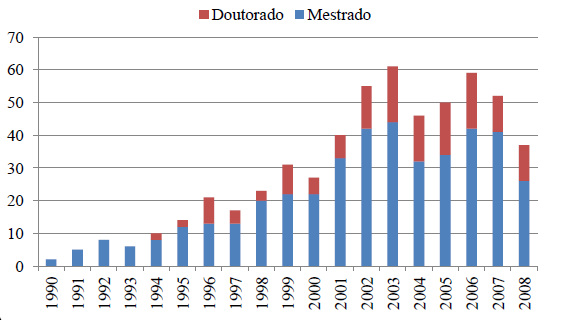
\includegraphics[scale=0.5]{figuras/figura-3}}
	}{
	\Fonte{os autores}
}
\end{figure}

Ou então figuras podem ser incorporadas de arquivos externos, como é o caso da \autoref{fig-grafico-1}. Se a figura que ser incluída se tratar de um diagrama, um gráfico ou uma ilustração que você mesmo produza, priorize o uso de imagens vetoriais no formato PDF. Com isso, o tamanho do arquivo final do trabalho será menor, e as imagens terão uma apresentação melhor, principalmente quando impressas, uma vez que imagens vetorias são perfeitamente escaláveis para qualquer dimensão. Nesse caso, se for utilizar o Microsoft Excel para produzir gráficos, ou o Microsoft Word para produzir ilustrações, exporte-os como PDF e os incorpore ao documento conforme o exemplo abaixo. No entanto, para manter a coerência no uso de software livre (já que você está usando LaTeX e abnTeX),  teste a ferramenta InkScape\index{InkScape}. ao CorelDraw\index{CorelDraw} ou ao Adobe Illustrator\index{Adobe! Illustrator}.  De todo modo, caso não seja possível  utilizar arquivos de imagens como PDF, utilize qualquer outro formato, como JPEG, GIF, BMP, etc.  Nesse caso, você pode tentar aprimorar as imagens incorporadas com o software livre \index{Gimp}Gimp. Ele é uma alternativa livre ao Adobe Photoshop\index{Adobe! Photoshop}.

\section{Usando Fórmulas Matemáticas}

\lipsum[2]

	\begin{equation}
		\begin{aligned}
			x = a_0 + \cfrac{1}{a_1
				+ \cfrac{1}{a_2
					+ \cfrac{1}{a_3 + \cfrac{1}{a_4} } } }
		\end{aligned}
	\end{equation}

\lipsum[3]

	\begin{equation}
		\begin{aligned}
			k_{n+1} = n^2 + k_n^2 - k_{n-1}
		\end{aligned}
	\end{equation}

\lipsum[4]

	\begin{equation}
		\begin{aligned}
			\cos (2\theta) = \cos^2 \theta - \sin^2 \theta
		\end{aligned}
	\end{equation}
	
\lipsum[5]

	\begin{equation}
		\begin{aligned}
			A_{m,n} =
			\begin{pmatrix}
			a_{1,1} & a_{1,2} & \cdots & a_{1,n} \\
			a_{2,1} & a_{2,2} & \cdots & a_{2,n} \\
			\vdots  & \vdots  & \ddots & \vdots  \\
			a_{m,1} & a_{m,2} & \cdots & a_{m,n}
			\end{pmatrix}
		\end{aligned}
	\end{equation}

\lipsum[6]

	\begin{equation}
		\begin{aligned}
			f(n) = \left\{ 
			\begin{array}{l l}
			n/2 & \quad \text{if $n$ is even}\\
			-(n+1)/2 & \quad \text{if $n$ is odd}
			\end{array} \right.
		\end{aligned}
	\end{equation}
	
\lipsum[7]

\section{Usando Algoritmos}

\lipsum[8]

\begin{algorithm}[h!]
	\SetSpacedAlgorithm
	\caption{\label{alg:algoritmo_de_colonica_de_formigas}Algoritmo de Otimização por Colônia de Formiga}
	\Entrada{Entrada do Algoritmo}
	\Saida{Saida do Algoritmo}
	\Inicio{
		Atribua os valores dos parâmetros\;
		Inicialize as trilhas de feromônios\;
		\Enqto{não atingir o critério de parada}{
			\Para{cada formiga}{
				Construa as Soluções\;
			}
			Aplique Busca Local (Opcional)\;
			Atualize o Feromônio\;
		}	
	}		
\end{algorithm}

\lipsum[9]

\section{Usando Código-fonte}

\lipsum[10]

\lstinputlisting[language=C++,caption={Hello World em C++}]{figuras/main.cpp}

\lipsum[11]

\begin{lstlisting}[language=Java,caption={Hello World em Java}]
public class HelloWorld {
	public static void main(String[] args) {
		System.out.println("Hello World!");
	}
}
\end{lstlisting}

\lipsum[11]

\section{Usando Teoremas, Proposições, etc}

Lorem ipsum dolor sit amet, consectetur adipiscing elit. Nunc dictum sed tortor nec viverra. consectetur adipiscing elit. Nunc dictum sed tortor nec viverra.

\begin{teo}[Pitágoras]
	Em todo triângulo retângulo o quadrado do comprimento da
	hipotenusa é igual a soma dos quadrados dos comprimentos dos catetos.
\end{teo}


Lorem ipsum dolor sit amet, consectetur adipiscing elit. Nunc dictum sed tortor nec viverra. consectetur adipiscing elit. Nunc dictum sed tortor nec viverra.

\begin{teo}[Fermat]
	Não existem inteiros $n > 2$, e $x, y, z$ tais que $x^n + y^n = z$
\end{teo}

Lorem ipsum dolor sit amet, consectetur adipiscing elit. Nunc dictum sed tortor nec viverra. consectetur adipiscing elit. Nunc dictum sed tortor nec viverra.

\begin{prop}
	Para demonstrar o Teorema de Pitágoras...
\end{prop}

Lorem ipsum dolor sit amet, consectetur adipiscing elit. Nunc dictum sed tortor nec viverra. consectetur adipiscing elit. Nunc dictum sed tortor nec viverra.

\begin{exem}
	Este é um exemplo do uso do ambiente exe definido acima.
\end{exem}

Lorem ipsum dolor sit amet, consectetur adipiscing elit. Nunc dictum sed tortor nec viverra. consectetur adipiscing elit. Nunc dictum sed tortor nec viverra.

\begin{xdefinicao}
	Definimos o produto de ...
\end{xdefinicao}

Lorem ipsum dolor sit amet, consectetur adipiscing elit. Nunc dictum sed tortor nec viverra. consectetur adipiscing elit. Nunc dictum sed tortor nec viverra.

\section{Usando Questões}


Lorem ipsum dolor sit amet, consectetur adipiscing elit. Nunc dictum sed tortor nec viverra. consectetur adipiscing elit. Nunc dictum sed tortor nec viverra.

\begin{questao}
	\item Esta é a primeira questão com alguns itens:
		\begin{enumerate}
			\item Este é o primeiro item
			\item Segundo item
		\end{enumerate}
	\item Esta é a segunda questão:
		\begin{enumerate}
			\item Este é o primeiro item
			\item Segundo item
		\end{enumerate}
	\item Lorem ipsum dolor sit amet, consectetur adipiscing elit. Nunc dictum sed tortor nec viverra. consectetur adipiscing elit. Nunc dictum sed tortor nec viverra.
		\begin{enumerate}
			\item consectetur
			\item adipiscing
			\item Nunc
			\item dictum
		\end{enumerate}
\end{questao}

\section{Citações}

\subsection{Documentos com três autores}

Quando houver três autores na citação, apresentam se os três, separados por ponto e vírgula, caso estes estejam após o texto. Se os autores estiverem incluídos no texto, devem ser separados por vírgula e pela conjunção "e".

\citeautoronline{tresautores}

\cite{tresautores}

\subsection{Documentos com mais de três autores}
Havendo mais de três autores, indica-se o primeiro seguido da expressão \textit{et al.} (do latim \textit{et alli}, que significa e outros), do ano e da página.

\citeautoronline{quatroautores}

\cite{quatroautores}

\subsection{Documentos de vários autores}

Havendo    citações    indiretas de    diversos    documentos    de    vários    autores, mencionados  simultaneamente e  que  expressam  a  mesma  ideia,  separam-se  os  autores  por ponto e vírgula, em ordem alfabética.

\cite{tresautores, quatroautores}

\section{Notas de Rodap\'{e}}

Deve-se utilizar o sistema autor-data para as  citações no texto e o numérico para notas explicativas\footnote{Veja - se como exemplo desse tipo de abordagem o estudo de Netzer (1976)}. As notas de rodapé podem e devem ser alinhadas, a partir da segunda linha da mesma nota, abaixo da primeira letra da primeira palavra, de forma a destacar o expoente \footnote{Encontramos  esse  tipo  de  perspectiva  na  2ª  parte  do  verbete  referido  na  nota  anterior,  em  grande  parte  do estudo de Rahner (1962).} e sem espaço entre elas e com fonte menor (tamanho 10).


	%\chapter{Resultados}
\label{chap:resultados}



\section{Resultados do Experimento A}
\label{sec:resultados-do-experimento-a}



\section{Resultados do Experimento B}
\label{sec:resultados-do-experimento-b}

	%\chapter{Conclusões e Trabalhos Futuros}
\label{chap:conclusoes-e-trabalhos-futuros}



\section{Contribuições do Trabalho}
\label{sec:contribuicoes-do-trabalho}



\section{Limitações}
\label{sec:limitacoes}


\section{Trabalhos Futuros}
\label{sec:trabalhos-futuros}






	%Elementos pós-textuais
	\bibliography{elementos-pos-textuais/referencias}
	%\imprimirglossario
	%\imprimirapendices
		% Adicione aqui os apendices do seu trabalho
		%\apendice{Lorem Ipsum}
\label{ap:lorem-ipsum}

\lipsum[1]
		%\apendice{Modelo de Capa}
\label{ap:modelo-de-capa}

\lipsum[1]

		%\apendice{Termo de Fiel Depositário}
\label{ap:termo-de-fiel-depositario}

\noindent \textbf{Pesquisa:} ANÁLISE DA MORTALIDADE INFANTIL COM MALFORMAÇÕES CONGÊNITAS.

\noindent Pelo presente instrumento que atende às exigências legais, a Sra. Maria Consuelo Martins Saraiva, ``fiel depositário'' com o cargo de Secretária Municipal de Saúde de Iracema, após ter tomado conhecimento do protocolo de pesquisa intitulado: ANÁLISE DA MORTALIDADE INFANTIL COM MALFORMAÇÕES CONGÊNITAS. Analisando a repercussão desse estudo no contexto da saúde pública e epidemiologia, autoriza Karla Maria da Silva Lima, enfermeira, aluna do Curso de Mestrado Acadêmico em Enfermagem da Universidade Estadual do Ceará (UECE), sob orientação do Prof. Dr. José Maria de Castro, da UECE, ter acesso aos bancos de dados do Sistema de Informação sobre Nascidos Vivos e do Sistema de Informação sobre Mortalidade da Secretaria Municipal de Saúde de Iracema, objeto deste estudo, e que se encontram sob sua total responsabilidade. Fica claro que o Fiel Depositário pode a qualquer momento retirar sua AUTORIZAÇÃO e ciente de que todas as informações prestadas tornar-se-ão confidenciais e guardadas por força de sigilo profissional, assegurando que os dados obtidos da pesquisa serão somente utilizados para estudo.
	%\imprimiranexos
		% Adicione aqui os anexos do seu trabalho
		%\anexo{Exemplo de Anexo}
\label{an:exemplo-de-anexo}

\lipsum[13]
		%\anexo{Dinâmica das classes sociais}
\label{an:dinamica-das-classes-sociais}

\lipsum[14]
\index{AAA}
	\imprimirindice

\end{document}
